\documentclass[../main.tex]{subfiles}

\begin{document}

\section{Introduction}

It is estimated that by 2020 there will be over 20 billion devices connected over the Internet \cite{gartner, juniper-research,stats-iot}. This collective of connected devices is called the Internet of Things (IoT)\nomenclature{IoT}{Internet of Things}. IoT systems can range from home monitoring, appliances and smart watches to smart hospitals and smart buildings. Some IoT systems can also be categorized as Cyber-Physical Systems (CPS)\nomenclature{CPS}{Cyber-Physical System}, such as the smart grid and smart healthcare \cite{ideas2020,els,k-ieee}. CPS are mission critical systems that interact with their surrounding environment \cite{shi2011survey, baheti2011cyber,banerjee2012ensuring}. IoT forms a foundation for Internet connected CPS \cite{k-ieee}. Figure~\ref{fig:iot-v-cps} shows the connection between IoT and CPS systems. As more devices become connected, there is a need to understand how the IoT and CPS Systems can rapidly scale, remain secure, and be resilient \cite{6803220,7275445}. 


\begin{figure}[!htb]
    \centering
    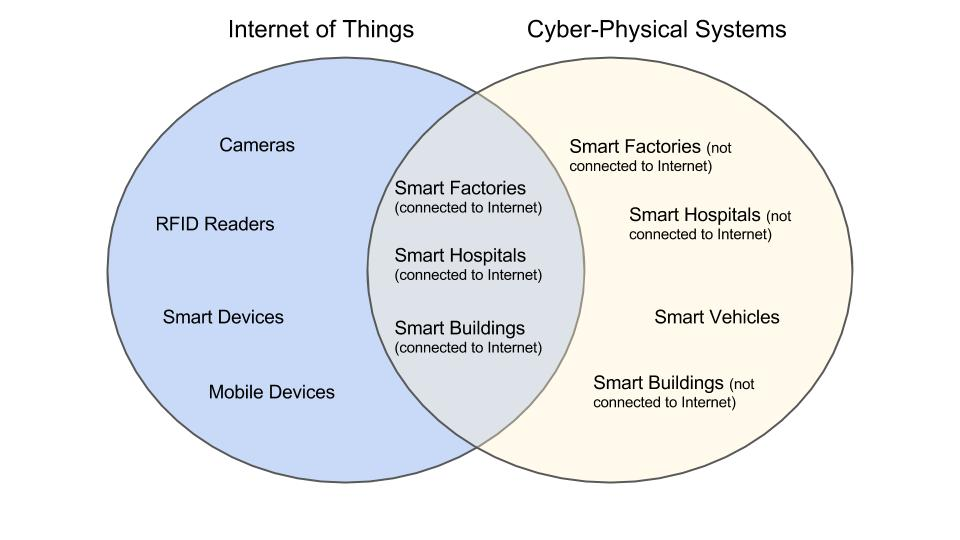
\includegraphics[scale=.35]{iotVScps.jpg}
    \caption{Internet of Things and Cyber-Physical Systems}
    \label{fig:iot-v-cps}
\end{figure}

Within an IoT/CPS systems devices can be divided into two primary groups: edge devices and gateway devices. Edge devices are low resource, simple devices that usually perform a single purpose, for instance reading ambient temperature. Gateway devices are more powerful than edge devices. They are used to aggregate data from edge devices and connect the edge devices to the Internet. Edge devices are connected to gateway devices to create IoT/CPS systems. One primary difference between IoT systems and CPS are CPS do not necessarily connect back to the Cloud. They can stand alone CPS of varying size from 10, 100, 1000, and 10000 devices. The goal of this dissertation is to address scalability, security, and resiliency separately and jointly in CPS architectures in an effort to create a robust, adaptable architecture. 

To accomplish our goal we propose a Multi-Tiered Resilient Architecture (M-TRA) \nomenclature{M-TRA}{Multi-Tiered Resilient Architecture}. The M-TRA would provide the foundation for a coalition of gateways to be formed. The coalition of gateways would allow for decision making to occur over a group of devices and no single device would maintain control over the entire system. When an edge device enters the CPS it sends a beacon message to find a gateway. The gateway that receives the beacon would collaborate with the coalition to determine if the new edge device can be trusted. If it is not trusted, they will alert the user and the device will not be allowed to enter the system. If it is trusted, the device will then be allowed in the system. The coalition of gateways will assign a primary gateway for the edge device to communicate with a secondary gateway as backup if the primary gateway goes down. These gateways will be determined based on reducing latency for transmission, balancing the load across the system, and distributing sensors in manner such that if a gateway does malfunction an entire sector of sensors does not disconnect. 

The remainder of this chapter is organized as follows: Section~\ref{sec:key-attributes} defines the key attributes of an IoT/CPS Architecture. Section~\ref{sec:tech-overview} overviews key technologies used in this dissertation. Section~\ref{sec:challenge} examines current challenges and opportunities. Section~\ref{sec:statement} is the statement of contribution provided in this dissertation. Section~\ref{sec:innovative} outlines our innovative claims. Finally, Section~\ref{sec:impact} overviews the broader impact associated with this dissertation.



\section{Key Architecture Attributes}
\label{sec:key-attributes}

There are three key attributes within a cohesive IoT/CPS Architectures for a robust system including security, scalability, and resiliency. Below we define and identify key points of each area. 

\subsection{Secure Architecture}
Within an IoT system, there are multiple levels of security including network security, secure device handshakes, and protection against intrusion into the devices. According to H\"oller, the Security Model for IoT consists of communication security that focuses mostly on the confidentiality and integrity protection of interacting entities, and functional components such as Identity Management, Authentication, Authorization, and Trust \& Reputation \cite{m2m_iot}.

The SANS Institute defines network security as “the process of taking physical and software preventative measures to protect the underlying networking infrastructure from unauthorized access, misuse, malfunction, modification, destruction, or improper disclosure, thereby creating a secure platform for computers, users and programs to perform their permitted critical functions within a secure environment." \cite{network_sans}

First, verifying the validity of a device before it is allowed to enter the system is fundamental for a trusted system. Secure device handshakes can provide this security to a system. For an IoT system, the handshake needs to be light-weight enough to run on end devices, yet robust enough to not be easily replicated or faked. Second, monitoring of each device is important to enable verification that a device has not become corrupt.

Along with security within the IoT system, if an intrusion or defect is detected, it is necessary to have the ability to determine who or what caused the failure. Digital Forensics can be implemented to provide a means to find this information. 

\subsection{Scalable Architecture}

When identifying scaling within an individual computer, there are two types of scaling: strong scaling and weak scaling. Strong scaling is CPU bound scaling. In strong scaling the problem size stays fixed while the number of processing elements are increased \cite{scaling}. Weak scaling is memory bound scaling. In this case the problem size (workload) assigned to each processing element stays constant and additional elements are used to solve a larger total problem (one that wouldn't fit in RAM on a single node, for example) \cite{scaling}. Scalability in parallel computing systems is the measure of its capacity to increase speedup in proportion to the increase in the number of processing elements \cite{parallel_computing}. 

Determining the speedup and efficiency within the systems as scaling occurs can be done by using Amdahl's law and Gustafson's law. Amdahl's law analyzes the speedup of a program given the addition of parallelization \cite{dr-dobbs}. Gustafson's law analyzes the increase in workload that can occur during a given time with the addition of parallelization. These two laws provide a foundation for determining the efficiency within the program is maximizing the use of the system. 


In IoT architecture, scalability includes scalability of operations within a gateway and scalability of increasing the number of devices included within the system. By analyzing weak and strong scaling within the gateway, we can investigate the ability to scale up the number of devices by using parallel processing with the CPU and GP-GPU. 

\subsection{Resilient Architecture}

According to Delic, Resiliency in an IoT system is defined in three parts \cite{Delic:2016:RIS:2891279.2822885}. First, an IoT system needs the ability to resist external perturbances and internal failures. Second, an IoT system should be capable of recovering and reentering a stable state after a failure occurs. Third, an IoT system should adapt its structure and behavior to constant change. 

\section{Overview of Technology}
\label{sec:tech-overview}
The following subsections provide an overview of each key area we explore with our work. 

\subfile{chapters/technology-overview.tex}{}

\section{Challenges and Opportunities}
\label{sec:challenge}
\subfile{chapters/challenge_opportunity.tex}{}

\section{Statement of Contributions}
\label{sec:statement}
\subfile{chapters/statement_of_contribution.tex}{}

\section{Innovative Claims}
\label{sec:innovative}
\subfile{chapters/innovative_claims.tex}{}

\section{Broader Impact}
\label{sec:impact}
\subfile{chapters/broader_impact.tex}{}



\end{document}